\documentclass[a4paper,11pt,twoside]{report}
\usepackage{amsmath}
\usepackage{ascmac}
\usepackage[dvipdfmx]{graphicx}  % for EPS and PDF 
\usepackage{url}
\usepackage{fancyvrb}
\usepackage{makeidx}
\usepackage{float}
\usepackage[dvipdfmx]{color}
\usepackage{vruler}  %% if vertical ruler (line number) is needed
\usepackage[dvipdfm,bookmarkstype=toc,urlcolor=black,%
    linkcolor=black,citecolor=black,bookmarks=false]{hyperref}
\setcounter{secnumdepth}{4}
\setcounter{tocdepth}{3}
\setcounter{totalnumber}{6}
\usepackage{fancyhdr}

\let\olditemize\itemize
\renewcommand{\itemize}{
   \olditemize
   \setlength{\itemsep}{8pt}
   \setlength{\parskip}{0pt}
   \setlength{\parsep}{0pt}
}

\parindent = 0pt
\hoffset=0cm
\oddsidemargin=0cm
\evensidemargin=0cm
\textwidth=16cm
\topmargin=-1cm
\voffset=0cm
\textheight=24cm

\long\def\comment#1{}
\def\progenv{\baselineskip=10pt\tt\progspecial{`}\parindent=0.3cm}
\def\shellenv{\baselineskip=10pt\tt\progspecial{`}\parindent=0.3cm\nolineno}

\renewcommand{\topfraction}{.99}
\renewcommand{\bottomfraction}{.99}

\def\openb{{\it [}}
\def\closeb{{\it ]}}
\def\DAG{$^\dagger$}
\def\DDAG{$^\ddagger$}
\def\XMP{XcalableMP}
\def\XACC{XcalableACC}
\def\OMP{OpenMP}
\def\OACC{OpenACC}
\def\HPF{HPF}
\def\CAF{Co-array Fortran}
\def\MPI{MPI}
\def\Fort{Fortran}
\def\C{C}
\def\XMPF{XcalableMP Fortran}
\def\XMPC{XcalableMP C}
\def\XACCF{XcalableACC Fortran}
\def\XACCC{XcalableACC C}
\def\Directive#1{{\tt #1}\index{#1@{\tt #1}}\index{Directive!#1@{\tt #1}}}
\def\Syntax#1{\index{Syntax!#1@{\tt #1}}}
\def\Term#1{{#1}\index{#1}}
\def\Example#1{\index{Example!#1@{\tt #1}}}
\def\Intrinsic#1{\index{#1@{\tt #1}}\index{Intrinsic and Library Procedures!#1@{\tt #1}}}
\def\NULL{{\tt NULL}}
\def\PROG#1{{\tt #1}\index{\tt #1}\index{Command!#1}}
\def\FUNC#1{{\tt #1()}\index{\tt #1}\index{Example Function!#1}}
\def\LPROG#1{{\tt #1}\index{\tt #1}\index{Linux Command!#1}}
\def\LFUNC#1{{\tt #1()}\index{\tt #1}\index{Linux Function!#1}}
\def\MFUNC#1{{\tt #1()}\index{\tt #1}\index{Myrinet/MX Function!#1}}
\def\SFUNC#1{{\tt #1()}\index{\tt #1}\index{Sample Code!#1}}
\def\STRUCT#1{{\tt #1}\index{\tt #1}\index{Struct!#1}}
\def\VAR#1{{\tt #1}\index{\tt #1}\index{Variable!#1}}
\def\ARG#1{{\tt #1}\index{\tt #1}\index{Variable!#1}}
\def\MACRO#1{{\tt #1}\index{\tt #1}\index{Macro!#1}}
\def\ERRNO#1{{\tt #1}\index{\tt #1}\index{ERRNO!#1}}
\def\SIGNAL#1{{\tt #1}\index{\tt #1}\index{Signal!#1}}
\def\FILE#1{{\tt #1}\index{\tt #1}\index{File!#1}}
\def\ENV#1{{\tt #1}\index{\tt #1}\index{Environment Variable!#1}}
\def\INDEX#1{#1\index{#1}}
\def\OPTION#1{{\tt #1}\index{Command Option!#1}}
\def\TERM#1{\underline{#1}\index{#1}}
\def\CTRL#1{{\tt $^\wedge$#1}}
\def\phrule{\vspace{0.2cm}\hrule\vspace{0.05cm}\hrule}
\def\qhrule{\vspace{0.2cm}\hrule}
\def\dhrule{\hrule\vspace{0.05cm}\hrule}
\def\bsquare{\rule[-2pt]{5pt}{10pt}}

\newcommand\gio{{\tt global\_io }}
\newcommand\mio{{\tt master\_io }}
\newcommand{\mytextcolor}[2]{{#2}}
\newcommand{\mycolor}[1]{\color{#1}}
\newenvironment{parcolor}[1]{\par\color{#1}}{\par}
\newenvironment{point}[1]{\vspace*{0.3cm}\begin{itembox}{#1}}{\end{itembox}\vspace*{0.3cm}}
\newenvironment{note}[1]{\vspace*{0.3cm}\begin{itembox}{Note on #1}}{\end{itembox}\vspace*{0.3cm}}
\newenvironment{issue}[1]{\vspace*{0.3cm}\begin{itembox}{Issues on #1}}{\end{itembox}\vspace*{0.3cm}}
\newenvironment{errors}{\vspace*{0.3cm}\begin{tabular}{ll}\multicolumn{2}{l}{\bf Return Values}\\}{\end{tabular}\vspace*{0.3cm}}
\newenvironment{mytable}[3]{\begin{table}[ht]\caption{#1}\label{#2}\vspace*{-0.3cm}\begin{center}\begin{tabular}{#3}}{\end{tabular}\end{center}\end{table}}
\newenvironment{myfigure}{\begin{figure}[ht]\begin{center}}{\end{center}\end{figure}}
%\DefineVerbatimEnvironment{FexampleL}{Verbatim}{numbers=left,numbersep=3pt,stepnumber=5,frame=single,label=\Fort}
%\DefineVerbatimEnvironment{FexampleR}{Verbatim}{numbers=right,numbersep=3pt,stepnumber=5,frame=single,label=\Fort}
%\DefineVerbatimEnvironment{Cexample}L{Verbatim}{numbers=left,numbersep=3pt,stepnumber=5,frame=single,label=\C}
%\DefineVerbatimEnvironment{CexampleR}{Verbatim}{numbers=right,numbersep=3pt,stepnumber=5,frame=single,label=\C}
%\DefineVerbatimEnvironment{XFexampleL}{Verbatim}{numbers=left,numbersep=3pt,stepnumber=5,frame=single,label=\XMPF}
%\DefineVerbatimEnvironment{XFexampleR}{Verbatim}{numbers=right,numbersep=3pt,stepnumber=5,frame=single,label=\XMPF}
%\DefineVerbatimEnvironment{XCexampleL}{Verbatim}{numbers=left,numbersep=3pt,stepnumber=5,frame=single,label=\XMPC}
%\DefineVerbatimEnvironment{XCexampleR}{Verbatim}{numbers=right,numbersep=3pt,stepnumber=5,frame=single,label=\XMPC}
%
\DefineVerbatimEnvironment{XACCCexampleR}{Verbatim}{numbers=right,numbersep=3pt,stepnumber=5,frame=single,label=\XACCC}
\DefineVerbatimEnvironment{XACCFexampleL}{Verbatim}{numbers=left,numbersep=3pt,stepnumber=5,frame=single,label=\XACCF}
%

\title{{\Huge XcalableACC}\\
$\langle${\it ex-scalable-a-c-c}$\rangle$\\
Language Specification\\
\vspace{2cm}
Version 1.0\\}
\author{
\Large RIKEN AICS and University of Tsukuba\\
}
\date{\vspace{4cm}\Large March 2017}

\makeindex

\begin{document}
\maketitle

Copyright \copyright 2017 Programming Environment Research Team of RIKEN AICS
and High Performance Computing System Laboratory of University of Tsukuba.
%Copyright \copyright 2016-2017 {\XMP} Specification Working Group.
%Permission to copy without fee all or part of this material is granted,
%provided the {\XMP} Specification Working Group copyright notice and the
%title of this document appear. Notice is given that copying is by permission
%of {\XMP} Specification Working Group.

\clearpage
%\setvruler[][][][3][0][1.2\textwidth]
\section*{History}

\paragraph*{Version 1.0: June 26, 2017}
First release.

\cleardoublepage

\pagenumbering{roman}
\tableofcontents

\newpage
\mbox{}\newpage

\pagestyle{fancy}
\fancyhead{} % clear all header fields
\fancyhead[RE]{\leftmark}
\fancyhead[LO]{\rightmark}
\fancyhead[LE,RO]{\thepage}
\fancyfoot{} % clear all footer fields
\renewcommand{\headrulewidth}{0pt}
\renewcommand{\footrulewidth}{0pt}

\chapter{Introduction}\label{chap:intro}
\pagenumbering{arabic}
\setcounter{page}{1}
This document defines the specification of {\XACC} which is an extension of {\XMP} version 1.3\cite{xmp} and {\OACC} version 2.5\cite{openacc}.
{\XACC} provides a parallel programming model for accelerated clusters
which are distributed memory systems equipped with accelerators.
In this document,
terminologies of {\XMP} and {\OACC} are indicated by {\bf bold font}.
For details, refer to each specification\cite{xmp,openacc}.

\section{Hardware Model}
The target of {\XACC} is an accelerated cluster,
a hardware model of which is shown in Fig. \ref{fig:hardware}.

\begin{myfigure}
  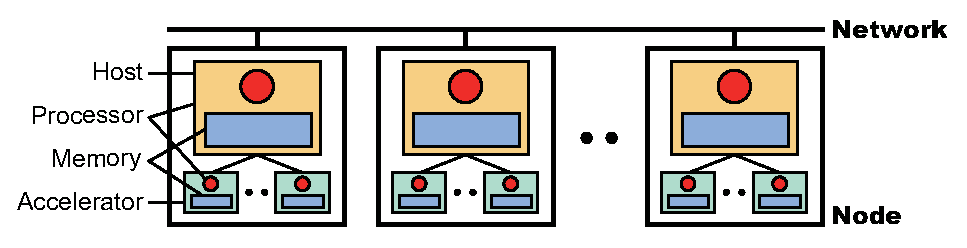
\includegraphics[scale=0.9,clip]{figs/hardware.eps}
  \caption{Hardware Model}\label{fig:hardware}
\end{myfigure}

An execution unit is called {\bf node} as with {\XMP}.
Each {\bf node} consists of a single host and multiple accelerators (such as GPUs and Intel MICs).
Each host has a processor, which may have several cores, and own local memory.
Each accelerator also has them.
Each {\bf node} is connected with each other via network.
Each {\bf node} can access its local memories directly and remote memories,
that is, the memories of another {\bf node} indirectly.
In a host,
the accelerator memory may be physically and/or virtually separate from the host memory as with the memory model of {\OACC}.
Thus,
a host may not be able to read or write the accelerator memory directly.

\section{Programming Model}
{\XACC} is a directive-based language extension based on Fortran 90 and ISO C90 (ANSI C90).
To develop applications on accelerated clusters with ease,
{\XACC} extends {\XACC} and {\OACC} independently as follow:
(1) {\XMP} extensions are to facilitate cooperation between {\XMP} and {\OACC} directives.
(2) {\OACC} extensions are to deal with multiple accelerators.

\subsection{{\XMP} Extensions}
In a program using the {\XMP} extensions,
{\XMP}, {\OACC}, and {\XACC} directives are used.
Fig. \ref{fig:concept} shows a concept of the {\XMP} extensions.

\begin{myfigure}
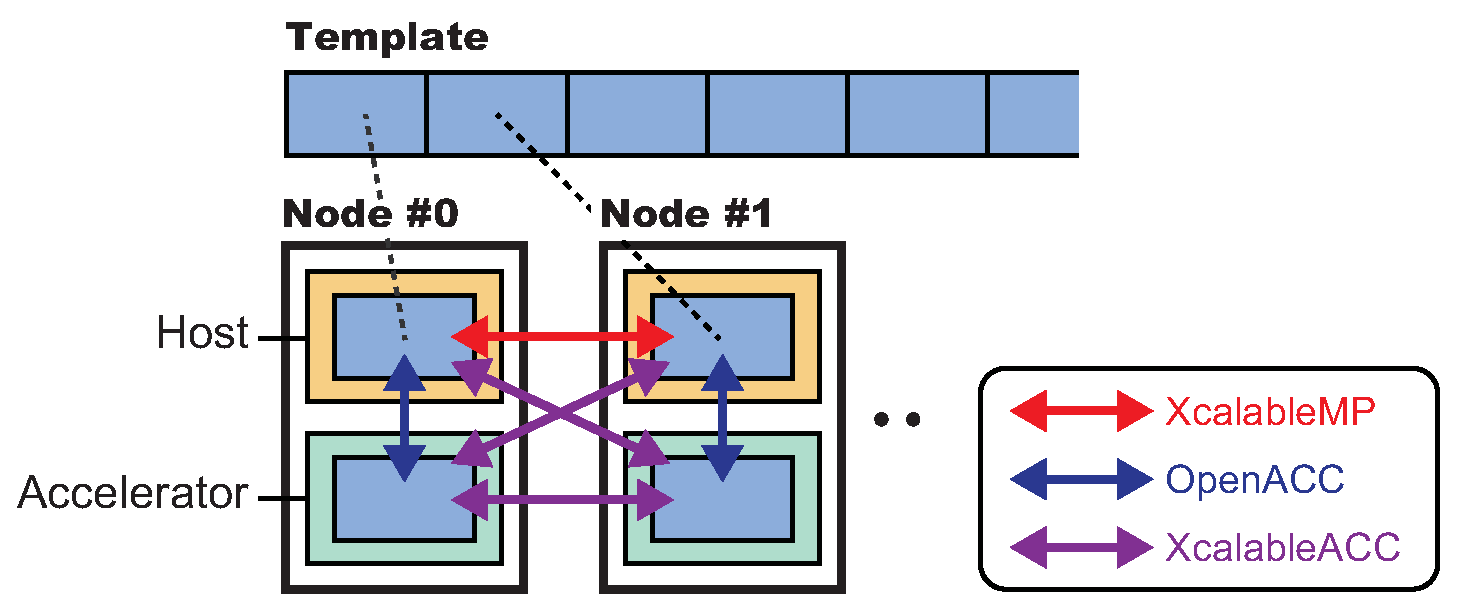
\includegraphics[scale=0.5,clip]{figs/concept.eps}
  \caption{Concept of {\XMP} Extensions}\label{fig:concept}
\end{myfigure}

{\XMP} directives define a {\bf template} and a {\bf node set}.
The {\bf template} represents a global index space, which is distributed onto the {\bf node set}.
Moreover, {\XMP} directives declare {\bf distributed arrays},
parallelize loop statements and transfer data among host memories according to the distributed {\bf template}.
{\OACC} directives transfer the {\bf distributed arrays} between host memory and accelerator memory on the same {\bf node}
and execute the loop statements parallelized by {\XMP} on accelerators in parallel.
{\XACC} directives, which are {\XMP} communication directives with an {\tt acc} clause, 
transfer data among accelerator memories and between accelerator memory and host memory on different {\bf nodes}.
Moreover, 
{\bf coarray} features also transfer data on different nodes.

%The {\XMP} extension is defined to develop parallel applications with keeping the sequential code image.
Note that 
the {\XMP} extensions are not a simple combination of {\XMP} and {\OACC}.
For example, 
if you represent communication of {\bf distributed array} among accelerators shown in Fig. \ref{fig:concept} by the combination of {\XMP} and {\OACC},
you need to specify explicitly communication between host and accelerator by {\OACC} and that between hosts by {\XMP}.
Moreover,
you need to calculate manually indices of the {\bf distributed array} owned by each {\bf node}.
By contrast,
{\XACC} directives can represent such communication among accelerators directly using global indices.

\subsection{{\OACC} Extensions}

\section{Execution Model}
The execution model of {\XACC} is a combination of those of {\XMP} and {\OACC}.
While the execution model of a host CPU programming is based on that of {\XMP},
that of an accelerator programming is based on that of {\OACC}.
Unless otherwise specified,
each {\bf node} behaves exactly as specified in the {\XMP} specification\cite{xmp} or the {\OACC} specification\cite{openacc}.
%For details, refer to each specification\cite{xmp,openacc}.

An {\XACC} program execution is based on the SPMD model, 
where each {\bf node} starts execution from the same main routine and keeps executing the same code independently (i.e. asynchronously), 
which is referred to as the replicated execution
until it encounters an {\XMP} construct or an {\XMP}-extension construct.
In particular,
the {\XMP}-extension construct may allocate, deallocate, or transfer data on accelerators.
An {\OACC} construct or an {\OACC}-extension construct may define {\bf parallel regions}, such as work-sharing loops, 
and offloads it to accelerators under control of the host.

When a {\bf node} encounters a loop construct 
targeted by a combination of {\XMP} {\tt loop} and {\OACC} {\tt loop} directives,
it executes the loop construct in parallel with other {\bf accelerators},
so that each iteration of the loop construct is independently executed by the {\bf accelerator}
where a specified data element resides.

When a {\bf node} encounters a {\XACC} synchronization or a {\XACC} communication directive,
synchronization or communication occurs between it and other accelerators.
That is, such {\bf global constructs} are performed collectively by the {\bf current executing nodes}.
Note that neither synchronizations nor communications occur without these constructs specified.

\section{Data Model}
There are two classes of data in {\XACC}: {\bf global data} and {\bf local data} as with {\XMP}. 
Data declared in an {\XACC} program are local by default.
Both {\bf global data} and {\bf local data} can exist on host memory and accelerator memory.
About the data models of host memory and accelerator memory, refer to the OpenACC specification\cite{openacc}.

{\bf Global data} are ones that are distributed onto the {\bf executing node set} by the {\tt align} directive.
Each fragment of a {\bf global data} is allocated in host memory of a {\bf node} in the {\bf executing node set}.
{\OACC} directives can transfer the fragment from host memory to accelerator memory.

{\bf Local data} are all of the ones that are not global.
They are replicated in the local memory of each of the {\bf executing nodes}.

A {\bf node} can access directly only {\bf local data} and sections of {\bf global data} that are allocated in its local memory.
To access data in remote memory, 
explicit communication must be specified in such ways as the global communication constructs and the {\bf coarray} assignments.

Particularly in {\XACCF}, 
for common blocks that include any global variables, 
the ways how the storage sequence of them is defined and how the storage association of them is resolved are implementation-dependent.

\section{Directive Format}
This section describes the syntax and behavior of {\XMP} and {\OACC} directives in {\XACC}.
In this document, 
the following notation is used to describe the directives.

\vspace{0.5cm}%
\begin{tabular}{ll}
{\tt xxx} & {\tt type-face} characters are used to indicate literal type characters. \\
{\it xxx...} & If the line is followed by ``...'', then xxx can be repeated. \\
{\it [xxx]} & {\it xxx} is optional. \\
{\bsquare} & The syntax rule continues. \\
\verb![F]! & The following lines are effective only in {\XACCF}. \\
\verb![C]! & The following lines are effective only in {\XACCC}. \\
\end{tabular}
\vspace{0.5cm}%

In {\XACCF}, 
{\XMP} and {\OACC} directives are specified using special comments that are identified by unique sentinels {\tt\verb|!$xmp|} and {\tt\verb|!$acc|} respectively.
the directives follow the rules for comment lines of either the Fortran free or fixed source form,
depending on the source form of the surrounding program unit\footnote{Consequently, the rules of comment lines that an
{\XMP} directive follows is the same as the ones that an {\OMP} directive follows.}.
The directives are case-insensitive.

\vspace{0.5cm}
\Syntax{directive}
\begin{tabular}{ll}
\verb![F]! & \verb|!$xmp| {\it directive-name clause} \\
\verb![F]! & \verb|!$acc| {\it directive-name clause} \\
\end{tabular}
\vspace{0.5cm}

In {\XACC}, 
{\XMP} and {\OACC} directives are specified using the \verb|#pragma| mechanism provided by the C standards.
the directives are case-sensitive.

\vspace{0.5cm}
\Syntax{directive}
\begin{tabular}{ll}
\verb![C]! & \verb|#pragma xmp| {\it directive-name clause} \\
\verb![C]! & \verb|#pragma acc| {\it directive-name clause} \\
\end{tabular}
\vspace{0.5cm}

%Directives are classified as {\bf declarative directives} and {\bf executable directives}\cite{xmp}.
%
%The {\bf declarative directives} are {\tt nodes}, {\tt template}, {\tt distribute}, {\tt align},
%{\tt shadow}, {\tt coarray}, {\tt declare}, and {\tt routine} directives.
%
%The {\bf executable directives} are {\tt template\_fix}, {\tt task}, {\tt tasks}, {\XMP} {\tt loop}, 
%{\tt array}, {\tt reflect}, {\tt reflect\_init}, {\tt reflect\_do}, {\tt gmove}, {\tt barrier}, 
%{\tt reduction}, {\tt bcast}, {\tt wait\_async},
%{\tt parallel}, {\tt kernels}, {\tt data}, {\tt host\_data}, {\OACC} {\tt loop},
%{\tt cache}, {\tt atomic}, {\tt init}, {\tt shutdown}, {\tt set}, {\tt update}, 
%{\tt wait}, {\tt enter\_data}, and {\tt exit\_data} directives.
%An {\bf executable directive} and its associated user code make up an {\XACC} construct, 
%as in the following format:
%
%\vspace{0.5cm}
%\begin{tabular}{ll}
%\verb![F]! & \verb|!$xmp| {\it directive-name clause} ...\\
% & \hspace{0.5cm} {\it structured-block} \\
%\verb![F]! & \verb|!$acc| {\it directive-name clause} ...\\
% & \hspace{0.5cm} {\it structured-block} \\
%\end{tabular}
%
%\vspace{0.3cm}
%
%\begin{tabular}{ll}
%\verb![C]! & \verb|#pragma xmp| {\it directive-name clause} ...\\
% & \hspace{0.5cm} {\it structured-block} \\
%\verb![C]! & \verb|#pragma acc| {\it directive-name clause} ...\\
% & \hspace{0.5cm} {\it structured-block} \\
%\end{tabular}
%\vspace{0.5cm}

\section{Organization of This Document}
The remainder of this document is structured as follows:

\begin{itemize}
 \item Chapter 2: {\XMP} Extensions
 \item Chapter 3: {\OACC} Extensions
\end{itemize}
 \cleardoublepage
\chapter{{\OACC} Extension}\label{chap:acc-ex}
 \cleardoublepage
\chapter{{\XMP} Extension}\label{chap:xmp-ex}
This chapter defines a behavior of mixing {\XMP} and {\OACC}.
Note that the existing {\OACC} is not extended in the {\XMP} extension.
The {\XMP} extension can represent 
(1) parallelization with keeping sequential code image using a combination of {\XMP} and {\OACC},
and
(2) communication among accelerator memories and between accelerator memory and host memory on different {\tt nodes}
using {\XACC} directives or {\tt coarray} features.

\section{Combination of {\XMP} and {\OACC}}
\subsection{{\OACC} Directives on Data}
\subsubsection*{Description}
When {\tt distributed arrays} appear in {\OACC} constructs,
global indices in {\tt distributed arrays} are used.
%Thus,
%an {\XACC} compiler automatically translates the global indices in the {\OACC} constructs to the appropriate local indices.
The {\tt distributed arrays} may appear in the {\OACC} {\bf update}, {\bf enter data}, {\bf exit data}, 
{\bf host\_data}, {\bf cache}, and {\bf declare} directives,
and the {\bf data} clause accompanied by some of 
{\bf deviceptr}, {\bf present}, {\bf copy}, {\bf copyin}, 
{\bf copyout}, {\bf create}, and {\bf delete} clauses.
Data transfer of {\tt distributed array} by {\OACC} is performed on only {\tt nodes} which have elements specified by the global indices.

\subsubsection*{Example}
\begin{myfigure}
\begin{minipage}{0.45\hsize}
\begin{center}
\begin{XACCFexampleL}
integer :: a(N), b(N)
!$xmp template t(N)
!$xmp nodes p(*)
!$xmp distribute t(block) onto p
!$xmp align a(i) with t(i)
!$xmp align b(i) with t(i)
...
!$acc enter data copyin(a(1:k))
!$acc data copy(b)
...
\end{XACCFexampleL}
\end{center}
\end{minipage}
%
\begin{minipage}{0.53\hsize}
\begin{center}
\begin{XACCCexampleR}
int a[N], b[N];
#pragma xmp template t[N]
#pragma xmp nodes p[*]
#pragma xmp distribute t[block] onto p
#pragma xmp align a[i] with t[i]
#pragma xmp align b[i] with t[i]
...
#pragma acc enter data copyin(a[0:k])
#pragma acc data copy(b)
{ ...
\end{XACCCexampleR}
\end{center}
\end{minipage}
\caption{Code example in {\XMP} extension with {\OACC} {\bf enter\_data} directive}\label{code:ex-oacc-data}
\end{myfigure}

In lines 2-6 of Fig. \ref{code:ex-oacc-data},
{\XMP} directives declare the {\tt distributed arrays} {\it a} and {\it b}.
In line 8,
the {\OACC} {\bf enter data} directive transfers the certain range of the {\tt distributed array} {\it a} from host memory to accelerator memory.
Note that the range is represented by global indices.
In line 9,
the {\OACC} {\bf data} directive transfers the whole {\tt distributed array} {\it b} from host memory to accelerator memory.

\subsection{{\OACC} Loop Construct}
\subsubsection*{Description}
In order to perform a loop statement on accelerators in {\tt nodes} in parallel,
{\XMP} {\bf loop} directive and {\OACC} {\bf loop} directive are used.
While
{\XMP} {\bf loop} directive performs a loop statement in {\tt nodes} in parallel,
{\OACC} {\bf loop} directive also performs the loop statement parallelized by the {\XMP} {\bf loop} directive 
on accelerators in parallel.
For ease of writing,
the order of {\XMP} {\bf loop} directive and {\OACC} {\bf loop} directive does not matter.

\subsubsection*{Restriction}
\begin{itemize}
\item In {\OACC} {\tt compute region},
only {\XMP} {\bf loop} directive without {\bf reduction} clause can be inserted.
\item In {\OACC} {\tt compute region},
targeted loop condition (lower bound, upper bound, and step of the loop)
must remain unchanged.
\end{itemize}

\subsubsection*{Example}
\begin{myfigure}
\begin{minipage}{0.45\hsize}
\begin{center}
\begin{XACCFexampleL}
integer :: a(N), b(N), sum = 0
!$xmp template t(N)
!$xmp nodes p(*)
!$xmp distribute t(block) onto p
!$xmp align a(i) with t(i)
!$xmp align b(i) with t(i)
...
!$acc parallel loop copy(a, b)
!$xmp loop on t(i)
do i=0, N
  b(i) = a(i)
end do
!$acc end parallel
\end{XACCFexampleL}
\end{center}
\end{minipage}
%
\begin{minipage}{0.53\hsize}
\begin{center}
\begin{XACCCexampleR}
int a[N], b[N], sum = 0;
#pragma xmp template t[N]
#pragma xmp nodes p[*]
#pragma xmp distribute t[block] onto p
#pragma xmp align a[i] with t[i]
#pragma xmp align b[i] with t[i]
...
#pragma acc parallel loop copy(a, b)
#pragma xmp loop on t[i]
for(int i=0;i<N;i++){
  b[i] = a[i];
}

\end{XACCCexampleR}
\end{center}
\end{minipage}
\caption{Code example in {\XMP} extension with {\OACC} loop construct}\label{code:ex-oacc-loop}
\end{myfigure}

In lines 2-6 of Fig. \ref{code:ex-oacc-loop},
{\XMP} directives declare {\tt distributed arrays} {\it a} and {\it b}.
In line 8,
{\OACC} {\bf parallel} directive with {\bf data} clause transfers the {\tt distributed arrays} {\it a} and {\it b} from host memory to accelerator memory.
Moreover,
in lines 8-9,
{\OACC} {\bf parallel} directive and {\XMP} {\bf loop} directive perform the next loop statement on accelerators in {\tt nodes} in parallel.

\section{Communication on Accelerated Clusters}
\subsection{{\XACC} Directives}
{\XACC} directives are extensions of {\XMP} {\bf reflect}, {\bf gmove}, 
{\bf barrier}, {\bf reduction}, {\bf bcast}, and {\bf wait\_async} directives in {\XMP} global-view memory model.
Moreover,
{\bf reflect\_init} and {\bf reflect\_do} directives are added as extensions of the {\bf reflect} directive.
When adding an {\bf acc} clause to the above directives,
data stored on accelerator memory are transferred.
Note that while XcalableACC {\bf gmove} directive described in Section \ref{sec:reflect} 
and {\tt coarray} features described in Section \ref{sec:coarray} can occur communication both among accelerator memories and between accelerator memory and host memory on different {\tt nodes},
other directives can occur communication only among accelerator memories.

This section describes only the extended parts of {\XACC} directives from {\XMP} directives. 
For other information, refer to the {\XMP} specification\cite{xmp}.

\subsubsection{reflect Construct}\label{sec:reflect}
\subsubsection*{Synopsis}
The {\bf reflect} construct assigns the value of a
reflection source to the corresponding shadow object.

\subsubsection*{Syntax}
\begin{tabular}{ll}
 \verb![F]! & \verb|!$xmp| {\tt reflect} \verb|(| {\it array-name}
 {\openb}, {\it array-name}{\closeb}... \verb|)| {\bsquare} \\
 &\hspace{0.1cm} {\bsquare} {\openb}{\tt width (} {\it reflect-width}
     {\openb}, {\it reflect-width}{\closeb}... {\tt )}{\closeb}
     {\openb}{\tt orthogonal}{\closeb}
     {\openb}{\tt async (} {\it async-id} {\tt )}{\closeb} {\openb}{\tt acc}{\closeb}\\
\verb![C]! & \verb|#pragma xmp| {\tt reflect} \verb|(| {\it array-name}
     {\openb}, {\it array-name}{\closeb}... \verb|)| {\bsquare} \\
 &\hspace{0.1cm} {\bsquare} {\openb}{\tt width (} {\it reflect-width}
     {\openb}, {\it reflect-width}{\closeb}... {\tt )}{\closeb}
     {\openb}{\tt orthogonal}{\closeb}
     {\openb}{\tt async (} {\it async-id} {\tt )}{\closeb} {\openb}{\tt acc}{\closeb}\\
\end{tabular}

\vspace{1em}
where {\it reflect-width} must be one of:
\vspace{1em}

\begin{tabular}{ll}
 \hspace{0.5cm} & {\openb}{\tt /periodic/}{\closeb} {\it int-expr} \\
                & {\openb}{\tt /periodic/}{\closeb} {\it int-expr} : {\it int-expr}
\end{tabular}

\subsubsection*{Description}
When the {\bf acc} clause is specified,
the {\bf reflect} construct updates each of the shadow object of the
array specified by {\it array-name} on accelerator memory with the value of its corresponding
reflection source.

\subsubsection*{Restriction}
\begin{itemize}
 \item When the {\bf acc} clause is specified,
   the arrays specified by the sequence of {\it array-name}'s must be allocated on accelerator memory.
 \item This construct must not appear in {\OACC} {\tt compute region}.
\end{itemize}

\subsubsection*{Example}
\begin{myfigure}
\begin{minipage}{0.45\hsize}
\begin{center}
\begin{XACCFexampleL}
integer :: a(N)
!$xmp template t(N)
!$xmp nodes p(*)
!$xmp distribute t(block) onto p
!$xmp align a(i) with t(i)
!$xmp shadow a(1)
...
!$acc enter data copyin(a)
!$xmp reflect (a) acc
\end{XACCFexampleL}
\end{center}
\end{minipage}
%
\begin{minipage}{0.53\hsize}
\begin{center}
\begin{XACCCexampleR}
int a[N];
#pragma xmp template t[N]
#pragma xmp nodes p[*]
#pragma xmp distribute t[block] onto p
#pragma xmp align a[i] with t[i]
#pragma xmp shadow a[1]
...
#pragma acc enter data copyin(a)
#pragma xmp reflect (a) acc
\end{XACCCexampleR}
\end{center}
\end{minipage}
\caption{Code example in {\XACC} {\bf reflect} construct}\label{code:reflect}
\end{myfigure}

In lines 2-5 of Fig. \ref{code:reflect},
{\XMP} directives declare {\tt distributed array} {\it a}.
In line 6, 
{\XMP} {\bf shadow} directive allocates shadow areas of the {\tt distributed array} {\it a}.
In line 8,
{\OACC} {\bf enter data} directive transfers the {\tt distributed array} {\it a} with the shadow areas from host memory to accelerator memory.
In line 9,
{\XACC} {\bf reflect} directive updates the shadow areas of the {\tt distributed array} {\it a} on accelerator memory between neighboring {\tt nodes}.

\subsubsection{reflect\_init and reflect\_do Constructs}\label{sec:gmove}
\subsubsection*{Synopsis}
Since the {\bf reflect\_init} construct performs the initialization processes of the {\bf reflect} construct,
the {\bf reflect\_do} construct performs communication of the {\bf reflect} construct.

\subsubsection*{Syntax}
\begin{tabular}{ll}
 \verb![F]! & \verb|!$xmp| {\tt reflect\_init} \verb|(| {\it array-name}
 {\openb}, {\it array-name}{\closeb}... \verb|)| {\bsquare} \\
 &\hspace{0.1cm} {\bsquare} {\openb}{\tt width (} {\it reflect-width}
     {\openb}, {\it reflect-width}{\closeb}... {\tt )}{\closeb}
     {\openb}{\tt orthogonal}{\closeb}
     {\openb}{\tt async (} {\it async-id} {\tt )}{\closeb} {\openb}{\tt acc}{\closeb}\\
\verb![C]! & \verb|#pragma xmp| {\tt reflect\_init} \verb|(| {\it array-name}
     {\openb}, {\it array-name}{\closeb}... \verb|)| {\bsquare} \\
 &\hspace{0.1cm} {\bsquare} {\openb}{\tt width (} {\it reflect-width}
     {\openb}, {\it reflect-width}{\closeb}... {\tt )}{\closeb}
     {\openb}{\tt orthogonal}{\closeb}
     {\openb}{\tt async (} {\it async-id} {\tt )}{\closeb} {\openb}{\tt acc}{\closeb}\\
\end{tabular}

\vspace{1em}
where {\it reflect-width} must be one of:
\vspace{1em}

\begin{tabular}{ll}
 \hspace{0.5cm} & {\openb}{\tt /periodic/}{\closeb} {\it int-expr} \\
                & {\openb}{\tt /periodic/}{\closeb} {\it int-expr} : {\it int-expr}
\end{tabular}

\vspace{1em}

\begin{tabular}{ll}
 \verb![F]! & \verb|!$xmp| {\tt reflect\_do} \verb|(| {\it array-name}
 {\openb}, {\it array-name}{\closeb}... \verb|)| {\openb}{\tt async (} {\it async-id} {\tt )}{\closeb} {\openb}{\tt acc}{\closeb}\\
\verb![C]! & \verb|#pragma xmp| {\tt reflect\_do} \verb|(| {\it array-name}
     {\openb}, {\it array-name}{\closeb}... \verb|)| 
     {\openb}{\tt async (} {\it async-id} {\tt )}{\closeb} {\openb}{\tt acc}{\closeb}\\
\end{tabular}

\subsubsection*{Description}
The {\bf reflect} construct is divided into {\bf reflect\_init} and {\bf reflect\_do} constructs to improve performance like the MPI persistent communication\cite{mpi}.

As a typical example, 
if a {\bf reflect} construct is called repeatedly with the same condition in a loop statement, 
inserting a {\bf reflect\_init} construct before the loop statement 
and replacing the {\bf reflect} construct with a {\bf reflect\_do} construct will improve its performance
because unneeded initialization processes are removed.

\subsubsection*{Restriction}
\begin{itemize}
 \item When the {\bf acc} clause is specified,
   the arrays specified by the sequence of {\it array-name}'s must be allocated on accelerator memory.
 \item These constructs must not appear in {\OACC} {\tt compute region}.
 \item The {\bf reflect\_init} directive must execute before the {\bf reflect\_init} directive executes.
\end{itemize}

\subsubsection*{Example}
\begin{myfigure}
\begin{minipage}{0.45\hsize}
\begin{center}
\begin{XACCFexampleL}
integer :: a(N)
!$xmp template t(N)
!$xmp nodes p(*)
!$xmp distribute t(block) onto p
!$xmp align a(i) with t(i)
!$xmp shadow a(1)
...
!$acc enter data copyin(a)
!$xmp reflect_init (a) acc
...
!$xmp reflect_do (a) acc
\end{XACCFexampleL}
\end{center}
\end{minipage}
%
\begin{minipage}{0.53\hsize}
\begin{center}
\begin{XACCCexampleR}
int a[N];
#pragma xmp template t[N]
#pragma xmp nodes p[*]
#pragma xmp distribute t[block] onto p
#pragma xmp align a[i] with t[i]
#pragma xmp shadow a[1]
...
#pragma acc enter data copyin(a)
#pragma xmp reflect_init (a) acc
...
#pragma xmp reflect_do (a) acc
\end{XACCCexampleR}
\end{center}
\end{minipage}
\caption{Code example in {\XACC} {\bf reflect\_init} and {\bf reflect\_do} constructs}\label{code:reflect_initdo}
\end{myfigure}

In lines 2-5 of Fig. \ref{code:reflect_initdo},
{\XMP} directives declare {\tt distributed array} {\it a}.
In line 6,
{\XMP} {\bf shadow} directive allocates shadow areas of the {\tt distributed array} {\it a}.
In line 8,
{\OACC} {\bf enter data} directive transfers the {\tt distributed array} {\it a} with the shadow areas from host memory to accelerator memory.
In line 9,
{\XACC} {\bf reflect\_init} directive performs initialization processes for the {\bf reflect\_do} construct which targets the {\tt distributed array} {\it a}.
In line 11,
{\XACC} {\bf reflect\_do} directive updates the shadow areas of the {\tt distributed array} {\it a} on accelerator memory between neighboring {\tt nodes}
without its initialization processes.

\subsubsection{gmove Construct}\label{sec:gmove}
\subsubsection*{Synopsis}
The {\tt \Directive{gmove}} construct allows an assignment statement,
which may cause communication, to be executed possibly in parallel by
the executing {\tt nodes}.

\subsubsection*{Syntax}
\begin{tabular}{ll}
\verb![F]! & \verb|!$xmp| {\tt gmove} {\openb}{\tt in} $\vert$ {\tt
 out}{\closeb} {\openb}{\tt async (} {\it async-id} {\tt )}{\closeb} {\openb}{\tt acc}{\openb}({\it variable}){\closeb}{\closeb}\\
\verb![C]! & \verb|#pragma xmp| {\tt gmove} {\openb}{\tt in} $\vert$ {\tt
 out}{\closeb} {\openb}{\tt async (} {\it async-id} {\tt )}{\closeb} {\openb}{\tt acc}{\openb}({\it variable}){\closeb}{\closeb}\\
\end{tabular}

\subsubsection*{Description}
\begin{itemize}
 \item When the {\bf acc} clause is specified and the variable is not specified by {\it variable} in the parenthesis,
variables of both sides in the assignment statement on accelerator memory are targeted.
 \item When the {\bf acc} clause is specified and the variable is specified by {\it variable} in the parenthesis,
the specified variable on accelerator memory is targeted, 
and the unspecified variable on host memory is targeted.
\end{itemize}

\subsubsection*{Restriction}
\begin{itemize}
 \item The variables targeted on accelerator memory must be allocated on accelerator memory.
 \item This construct must not appear in {\OACC} {\tt compute region}.
\end{itemize}

\subsubsection*{Example}
\begin{myfigure}
\begin{minipage}{0.45\hsize}
\begin{center}
\begin{XACCFexampleL}
integer :: a(N), b(N)
!$xmp template t(N)
!$xmp nodes p(*)
!$xmp distribute t(block) onto p
!$xmp align a(i) with t(i)
!$xmp align b(i) with t(i)
...
!$acc enter data copyin(a, b)
!$xmp gmove acc
  a(:) = b(:)

!$xmp gmove acc(b)
  a(:) = b(:)
\end{XACCFexampleL}
\end{center}
\end{minipage}
%
\begin{minipage}{0.53\hsize}
\begin{center}
\begin{XACCCexampleR}
int a[N], b[N];
#pragma xmp template t[N]
#pragma xmp nodes p[*]
#pragma xmp distribute t[block] onto p
#pragma xmp align a[i] with t[i]
#pragma xmp align b[i] with t[i]
...
#pragma acc enter data copyin(a, b)
#pragma xmp gmove acc
  a[:] = b[:];

#pragma xmp gmove acc(b)
  a[:] = b[:];
\end{XACCCexampleR}
\end{center}
\end{minipage}
\caption{Code example in {\XACC} {\bf gmove} construct}\label{code:gmove}
\end{myfigure}

In lines 2-6 of Fig. \ref{code:gmove},
{\XMP} directives declare {\tt distributed arrays} {\it a} and {\it b}.
In line 8,
{\OACC} {\bf enter data} directive transfers the {\tt distributed arrays} {\it a} and {\it b} from host memory to accelerator memory.
In lines 9-10,
{\XACC} {\bf gmove} construct copies the whole {\tt distributed array} {\it b} to
that of the {\tt distributed array} {\it a} on accelerator memories.
In lines 12-13,
{\XACC} {\bf gmove} construct copies the whole {\tt distributed array} {\it b} on accelerator memory to
that of the {\tt distributed array} {\it a} on host memory.

\subsubsection{barrier Construct}\label{sec:barrier}
\subsubsection*{Synopsis}
The {\bf barrier} construct specifies an explicit barrier
at the point at which the construct appears.

\subsubsection*{Syntax}
\begin{tabular}{ll}
\verb![F]! & \verb|!$xmp| {\tt barrier} {\openb}{\tt on} {\it nodes-ref}
 $\vert${\it template-ref}{\closeb} {\openb}{\tt acc}{\closeb}\\
\verb![C]! & \verb|#pragma xmp| {\tt barrier} {\openb}{\tt on} {\it
     nodes-ref} $\vert$ {\it template-ref}{\closeb} {\openb}{\tt acc}{\closeb}\\
\end{tabular}

\subsubsection*{Description}
\begin{itemize}
 \item When the {\bf acc} clause is specified,
the barrier construct blocks until all outgoing asynchronous operations on accelerators are completed.
 \item When the {\bf acc} clause is not specified,
the barrier construct does not guarantee that an outgoing asynchronous operation on accelerator is completed.
\end{itemize}

\subsubsection*{Example}
\begin{myfigure}
\begin{minipage}{0.45\hsize}
\begin{center}
\begin{XACCFexampleL}
!$xmp nodes p(*)
...
!$xmp barrier acc
\end{XACCFexampleL}
\end{center}
\end{minipage}
%
\begin{minipage}{0.53\hsize}
\begin{center}
\begin{XACCCexampleR}
#pragma xmp nodes p[*]
...
#pragma xmp barrier acc
\end{XACCCexampleR}
\end{center}
\end{minipage}
\caption{Code example in {\XACC} {\bf barrier} construct}\label{code:barrier}
\end{myfigure}

In line 1,
{\XMP} {\bf nodes} directive defines {\tt node set} {\it p}.
In line 3,
{\XACC} {\bf barrier} directive performs a barrier operation for accelerators on all {\tt node}.

\subsubsection{reduction Construct}\label{sec:reduction}
\subsubsection*{Synopsis}
The {\bf reduction} construct performs a reduction operation among {\tt nodes}.

\subsubsection*{Syntax}
\Syntax{reduction}

\begin{tabular}{ll}
\verb![F]! & \verb|!$xmp| {\tt reduction (} {\it reduction-kind} {\it
  :} {\it variable} {\openb}, {\it variable} {\closeb}... {\tt )}
 {\bsquare} \\
 & \hspace{5cm} {\bsquare} {\openb}{\tt on} {\it node-ref} $\vert$ {\it
     template-ref}{\closeb} {\openb}{\tt async (} {\it async-id} {\tt )}{\closeb} {\openb}{\tt acc}{\closeb}\\
\end{tabular}

\vspace{0.5cm}
where {\it reduction-kind} is one of:

\begin{tabular}{ll}
 \hspace{0.5cm} & {\tt +} \\
 & {\tt *} \\
% & {\tt -} \\
 & {\tt .and.} \\
 & {\tt .or.} \\
 & {\tt .eqv.} \\
 & {\tt .neqv.} \\
 & {\tt max} \\
 & {\tt min} \\
 & {\tt iand} \\
 & {\tt ior} \\
 & {\tt ieor} \\
\end{tabular}

\vspace{0.5cm}

\begin{tabular}{ll}
 \hspace{-\parindent}
 \verb![C]! & \verb|#pragma xmp| {\tt reduction (} {\it reduction-kind} {\it
  :} {\it variable} {\openb}, {\it variable} {\closeb}... {\tt )}
 {\bsquare} \\
 & \hspace{5cm} {\bsquare} {\openb}{\tt on} {\it node-ref} $\vert$ {\it
     template-ref}{\closeb} {\openb}{\tt async (} {\it async-id} {\tt )}{\closeb} {\openb}{\tt acc}{\closeb} \\
\end{tabular}
\vspace{0.5cm}

where {\it reduction-kind} is one of:

\begin{tabular}{ll}
 \hspace{0.5cm} & {\tt +} \\
 & {\tt *} \\
% & {\tt -} \\
 & {\verb|&|} \\
 & {\tt |} \\
 & {\verb|^|} \\
 & {\verb|&&|} \\
 & {\tt ||} \\
 & {\tt max} \\
 & {\tt min} \\
\end{tabular}

\subsubsection*{Description}
When the {\bf acc} clause is specified,
the {\tt reduction} construct performs a type of
reduction operation specified by {\it reduction-kind} for the specified
local variables among the accelerators and 
sets the reduction results to the variables on each of the accelerators.

\subsubsection*{Restriction}
\begin{itemize}
 \item When the {\bf acc} clause is specified,
   the variables specified by the sequence of {\it variable}'s must be allocated on accelerator memory.
 \item This construct must not appear in {\OACC} {\tt compute region}.
\end{itemize}

\subsubsection*{Example}
\begin{myfigure}
\begin{minipage}{0.45\hsize}
\begin{center}
\begin{XACCFexampleL}
integer :: a
!$xmp nodes p(*)
...
!$acc enter data copyin(a)
!$xmp reduction(+:a) acc
\end{XACCFexampleL}
\end{center}
\end{minipage}
%
\begin{minipage}{0.53\hsize}
\begin{center}
\begin{XACCCexampleR}
int a;
#pragma xmp nodes p[*]
...
#pragma acc enter data copyin(a)
#pragma xmp reduction(+:a) acc
\end{XACCCexampleR}
\end{center}
\end{minipage}
\caption{Code example in {\XACC} {\bf reduction} construct}\label{code:reduction}
\end{myfigure}

In line 2,
{\XMP} {\bf nodes} directive defines {\tt node set} {\it p}.
In line 4,
{\OACC} {\bf enter data} directive transfers the local variable {\it a} from host memory to accelerator memory.
In line 5,
{\XACC} {\bf reduction} directive calculates a total value of the variable {\it a} stored on each accelerator
memory in each {\tt node}.

\subsubsection{bcast Construct}\label{sec:bcast}
\subsubsection*{Synopsis}
The {\bf bcast} construct performs broadcast communication from a specified {\tt node}.

\subsubsection*{Syntax}

\begin{tabular}{ll}
 \verb![F]! & \verb|!$xmp| {\tt bcast} \verb|(| {\it variable}
 {\openb}, {\it variable}{\closeb}... \verb|)|
 {\openb}{\tt from} {\it nodes-ref} $\vert$ {\it template-ref}{\closeb}
 {\bsquare} \\
 & \hspace{4.8cm} {\bsquare} {\openb}{\tt on} {\it nodes-ref}{\closeb}
     $\vert$ {\it template-ref}{\closeb}
     {\openb}{\tt async (} {\it async-id} {\tt )}{\closeb} {\openb}{\tt acc}{\closeb}\\

 \verb![C]! & \verb|#pragma xmp| {\tt bcast} \verb|(| {\it variable}
 {\openb}, {\it variable}{\closeb}... \verb|)|
 {\openb}{\tt from} {\it nodes-ref}  $\vert$ {\it
     template-ref}{\closeb} {\bsquare} \\
 & \hspace{4.8cm} {\bsquare} {\openb}{\tt on} {\it nodes-ref} $\vert$ {\it
     template-ref}{\closeb}
 {\openb}{\tt async (} {\it async-id} {\tt )}{\closeb} {\openb}{\tt acc}{\closeb}\\
\end{tabular}

\subsubsection*{Description}
When the {\bf acc} clause is specified, 
the values of the variables specified by the sequence of {\it variable}'s on accelerator memory
(called {\tt broadcast variables}) are broadcasted
from the {\tt node} specified by the {\tt from} clause (called the
{\tt source node}) to each of the {\tt nodes} in the {\tt node set} specified
by the {\tt on} clause. After executing this construct,
the values of the {\tt broadcast variables} become the same as those in the {\tt source node}.

\subsubsection*{Restriction}
\begin{itemize}
 \item When the {\bf acc} clause is specified,
   the variables specified by the sequence of {\it variable}'s must be allocated on accelerator memory.
 \item This construct must not appear in {\OACC} {\tt compute region}.
\end{itemize}

\subsubsection*{Example}
\begin{myfigure}
\begin{minipage}{0.45\hsize}
\begin{center}
\begin{XACCFexampleL}
integer :: a
!$xmp nodes p(*)
...
!$acc enter data copyin(a)
!$xmp bcast(a) acc
\end{XACCFexampleL}
\end{center}
\end{minipage}
%
\begin{minipage}{0.53\hsize}
\begin{center}
\begin{XACCCexampleR}
int a;
#pragma xmp nodes p[*]
...
#pragma acc enter data copyin(a)
#pragma xmp bcast(a) acc
\end{XACCCexampleR}
\end{center}
\end{minipage}
\caption{Code example in {\XACC} {\bf bcast} construct}\label{code:bcast}
\end{myfigure}

In line 2,
{\XMP} {\bf nodes} directive defines {\tt node set} {\it p}.
In line 4,
{\OACC} {\bf enter data} directive transfers the local variable {\it a} from host memory to accelerator memory.
In line 5,
{\XACC} {\bf bcast} directive broadcasts the variable {\it a} stored on accelerator memory to all {\it nodes}.

\subsubsection{wait\_async Construct}\label{sec:waitasync}
\subsubsection*{Synopsis}
The {\bf wait\_async} construct guarantees asynchronous
communications specified by {\it async-id} are complete.

\subsubsection*{Syntax}
\begin{tabular}{ll}
\verb![F]! & \verb|!$xmp| {\tt wait\_async ( {\it async-id} {\openb},
 {\it async-id} {\closeb}...)} {\openb}{\tt on} {\it nodes-ref} $\vert$
 {\it template-ref}{\closeb} {\openb}{\tt acc}{\closeb}\\
\verb![C]! & \verb|#pragma xmp| {\tt wait\_async ( {\it async-id} {\openb},
 {\it async-id} {\closeb}...)} {\openb}{\tt on} {\it nodes-ref} $\vert$
 {\it template-ref}{\closeb} {\bsquare} \\
& \hspace{13.5cm} {\bsquare} {\openb}{\tt acc}{\closeb}\\
\end{tabular}

\subsubsection*{Description}
When the {\bf acc} clause is specified,
the {\bf wait\_async} construct blocks and therefore
statements following it are not executed until all of the asynchronous
communications that are specified by {\it async-id}'s and issued on the accelerators in
{\tt node set} specified by the {\tt on} clause are complete.

\subsubsection*{Restriction}
This construct must not appear in {\OACC} {\tt compute region}.

\subsubsection*{Example}
\begin{myfigure}
\begin{minipage}{0.45\hsize}
\begin{center}
\begin{XACCFexampleL}
integer :: a
!$xmp nodes p(*)
...
!$acc enter data copyin(a)
!$xmp reduction(+:a) acc async(1)
...
!$xmp wait_async(1) acc
\end{XACCFexampleL}
\end{center}
\end{minipage}
%
\begin{minipage}{0.53\hsize}
\begin{center}
\begin{XACCCexampleR}
int a;
#pragma xmp nodes p[*]
...
#pragma acc enter data copyin(a)
#pragma xmp reduction(+:a) acc async(1)
...
#pragma xmp wait_async(1) acc
\end{XACCCexampleR}
\end{center}
\end{minipage}
\caption{Code example in {\XACC} {\bf wait\_async} construct}\label{code:waitasync}
\end{myfigure}

In line 2,
{\XMP} {\bf nodes} directive defines {\tt node set} {\it p}.
In line 4,
{\OACC} {\bf enter data} directive transfers the local variable {\it a} from host memory to accelerator memory.
In line 5,
{\XACC} {\bf reduction} directive performs asynchronously.
In line 7,
{\XACC} {\bf wait\_async} construct blocks until the asynchronous {\bf reduction} operation at line 5 is complete.

\subsection{Coarray Features} \label{sec:coarray}
\subsubsection*{Synopsis}
{\XACC} can perform one-sided communication (put/get operations) for data on accelerator memory using {\tt coarray} features,
which is based on {\XMP} local-view memory model.
A combination of {\tt coarray} syntax and {\OACC} {\bf host\_data} construct enables communication between accelerators.

\subsubsection*{Description}
If {\tt coarrays} appear in {\OACC} {\bf use\_device} clause of any {\OACC} enclosing {\bf host\_data} construct, 
communication targets data on the accelerator side. 
{\tt Coarray} operations on accelerators are synchronized using the same synchronization functions in {\XMP}.

\subsubsection*{Restriction}
\begin{itemize}
 \item Only {\OACC} {\bf declare} directive can declare a {\tt coarray} on accelerator memory.
   For example,
   {\OACC} {\bf enter data} and {\bf copy} directives cannot declare a {\tt coarray} on accelerator memory.
 \item The {\tt coarray} syntax must not appear in {\OACC} {\tt compute region}.
\end{itemize}

\subsubsection*{Example}
\begin{myfigure}
\begin{minipage}{0.45\hsize}
\begin{center}
\begin{XACCFexampleL}
integer :: a(N)[*]
integer :: b(N)
!$acc declare create(a, b)
...
if(this_image() == 1) then
!$acc host_data use_device(a, b)
  a(:)[2] = b(:)

!$acc host_data use_device(a)
  b(:) = a(:)[3]
end if
...
sync all
\end{XACCFexampleL}
\end{center}
\end{minipage}
%
\begin{minipage}{0.53\hsize}
\begin{center}
\begin{XACCCexampleR}
int a[N]:[*];
int b[N];
#pragma acc declare create(a, b)
...
if(xmp_node_num() == 1){
#pragma acc host_data use_device(a, b)
  a[:]:[2] = b[:];

#pragma acc host_data use_device(a)
  b[:] = a[:]:[3];
}
...
xmp_sync_all(NULL);
\end{XACCCexampleR}
\end{center}
\end{minipage}
\caption{Code example in {\XACC} coarray features}\label{code:coarray}
\end{myfigure}

In line 3 of Fig. \ref{code:coarray},
{\OACC} {\bf declare} directive declares a {\tt coarray} {\it a} and a array {\it b} on accelerator memory.
In lines 6-7,
{\tt node} 1 performs put operation, where
the whole array {\it b} on accelerator memory in {\tt node} 1 is transferred to the {\tt coarray} {\it a} on accelerator memory in {\tt node} 2.
In lines 9-10,
{\tt node} 1 performs get operation, where
the whole {\tt coarray} {\it a} on accelerator memory in {\tt node} 3 is transferred to the array {\it b} on host memory in {\tt node} 1.
In line 13,
the {\bf sync all} statement in {\XACCF} or the {\bf xmp\_sync\_all} function in {\XACCC} synchronizes all {\tt nodes} and guarantees completion of ongoing coarray operations.

 \cleardoublepage
%\input{glossary.tex

\cleardoublepage
\chapter*{Acknowledgment}
%\begin{itemize}
%\setlength{\itemsep}{-1mm}
%\item Taisuke Boku       \dotfill \ University of Tsukuba
%\item Hidetoshi Iwashita \dotfill \ RIKEN/Fujitsu Inc.
%\item Hitoshi Murai      \dotfill \ RIKEN
%\item Masahiro Nakao     \dotfill \ RIKEN
%\item Mitsuhisa Sato     \dotfill \ RIKEN
%\item Akihiro Tabuchi     \dotfill \ University of Tsukuba
%\end{itemize}

The work was supported by the Japan Science and Technology Agency, 
Core Research for Evolutional Science and Technology program entitled 
``Research and Development on Unified Environment of Accelerated Computing and Interconnection for Post-Petascale Era'' 
in the research area of ``Development of System Software Technologies for Post-Peta Scale High Performance Computing.''

%The specification of {\XMP} is designed by the {\XMP} Specification
%Working Group, which consists of the following members from academia,
%research laboratories, and industries.

\begin{thebibliography}{99}
\addcontentsline{toc}{chapter}{\bibname}
 \bibitem{xmp} XcalableMP Language Specification, \url{http://xcalablemp.org/specification.html} (2017).
 \bibitem{openacc} The OpenACC Application Programming Interface, \url{http://www.openacc.org} (2015).
 \bibitem{mpi} MPI: A Message-Passing Interface Standard, \url{http://mpi-forum.org} (2015).
\end{thebibliography}

\end{document}
